\setcounter{exo}{0}

Soit le schéma-blocs suivant.
\begin{center}
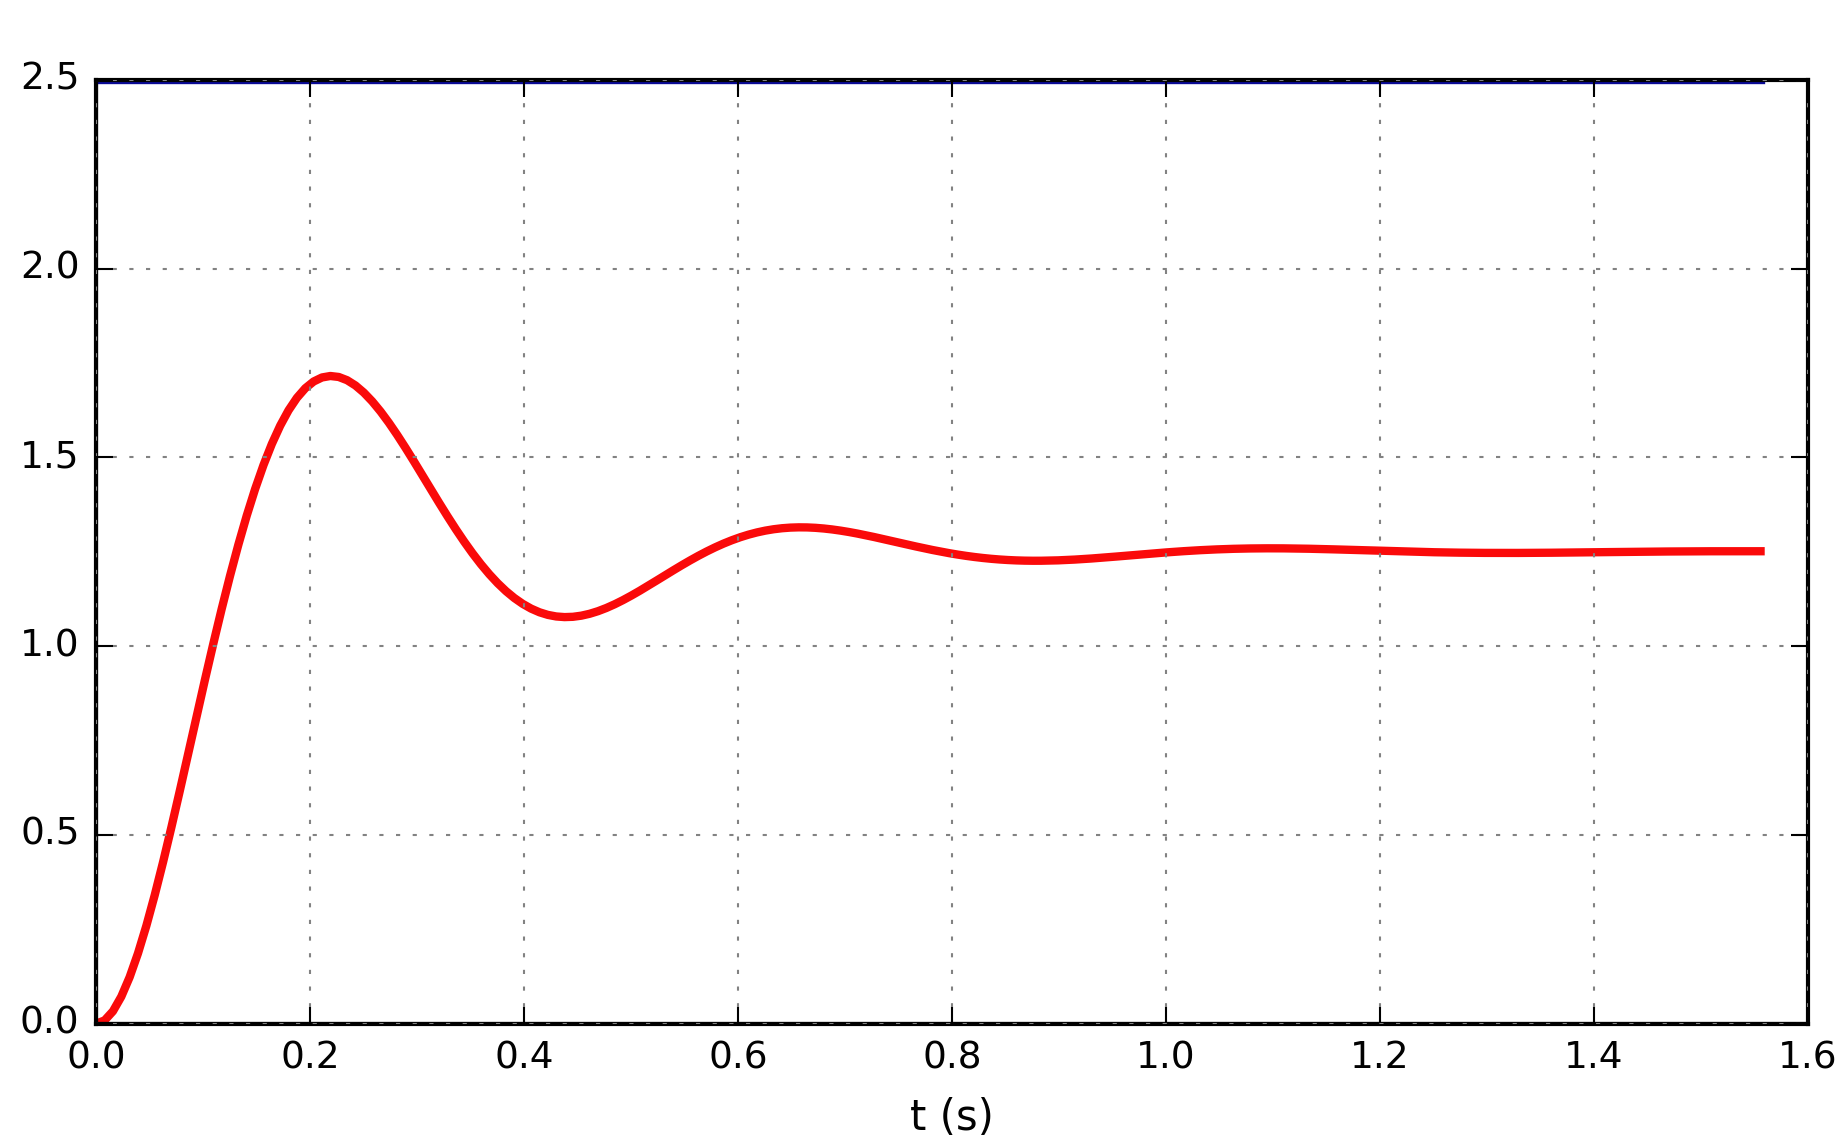
\includegraphics[width=.9\linewidth]{fig_02}
\end{center}

\subparagraph{}
\textit{Déterminer la fonction de transfert en boucle fermée. Mettre l'expression sous forme canonique et exprimer les paramétres caractéristiques.}


Soit le schéma-blocs suivant.
\begin{center}
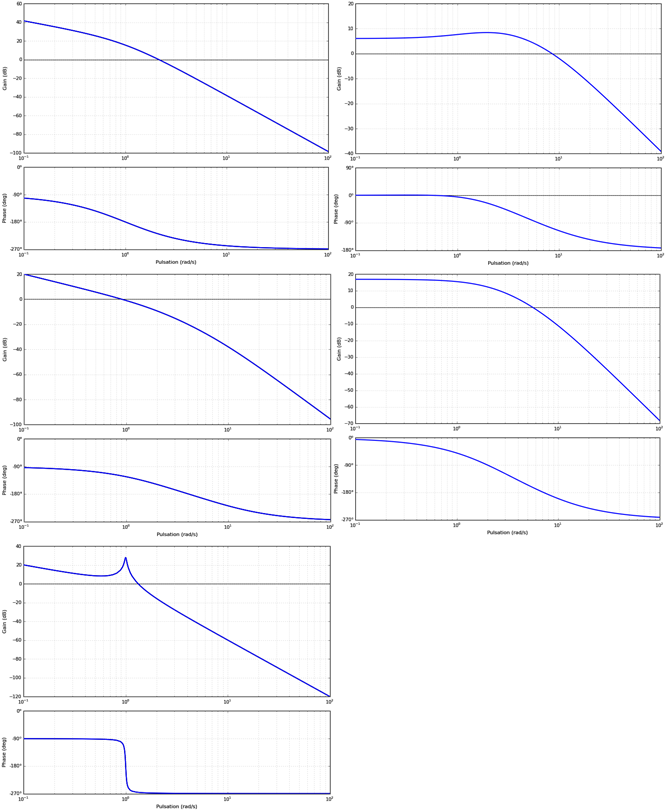
\includegraphics[width=.9\linewidth]{fig_01}
\end{center}

\subparagraph{}
\textit{Déterminer la fonction de transfert en boucle fermée. Mettre l'expression sous forme canonique et exprimer les paramétres caractéristiques.}